\documentclass[12pt,a4paper]{article}

\usepackage[utf8]{inputenc}
\usepackage[T2A]{fontenc}
\usepackage[russian]{babel}
\usepackage{amsmath}
\usepackage{amssymb}
\usepackage{array}
\usepackage{booktabs}
\usepackage{caption}
\usepackage{enumitem}
\usepackage{fancyhdr}
\usepackage{float}
\usepackage{geometry}
\usepackage{graphicx}
\usepackage{hyperref}
\usepackage{indentfirst}
\usepackage{listings}
\usepackage{longtable}
\usepackage{xcolor}

\geometry{left=30mm,right=15mm,top=20mm,bottom=20mm}
\setlength{\parindent}{1.25cm}
\linespread{1.2}
\pagestyle{fancy}
\fancyhf{}
\fancyfoot[C]{\thepage}
\renewcommand{\headrulewidth}{0pt}
\hypersetup{hidelinks}

\captionsetup{justification=centering}
\setcounter{tocdepth}{2}

\definecolor{codebg}{RGB}{248,248,248}
\definecolor{codeframe}{RGB}{215,215,215}
\definecolor{codekw}{RGB}{0,76,153}
\definecolor{codestr}{RGB}{163,21,21}
\definecolor{codecomment}{RGB}{0,128,0}

\lstdefinelanguage{JavaScript}{
  morekeywords={const,let,var,function,return,if,else,for,while,throw,new,export,import,from,class,get},
  sensitive=true,
  morecomment=[l]{//},
  morestring=[b]",
  morestring=[b]',
}

\lstset{
  language=JavaScript,
  basicstyle=\ttfamily\small,
  keywordstyle=\color{codekw}\bfseries,
  stringstyle=\color{codestr},
  commentstyle=\color{codecomment},
  backgroundcolor=\color{codebg},
  frame=single,
  rulecolor=\color{codeframe},
  numbers=left,
  numberstyle=\tiny,
  stepnumber=1,
  breaklines=true,
  showstringspaces=false,
  tabsize=2,
  columns=fullflexible,
  keepspaces=true,
  extendedchars=true,
  inputencoding=utf8
}

\newcolumntype{C}[1]{>{\centering\arraybackslash}p{#1}}

\begin{document}

% ====================== ТИТУЛЬНЫЙ ЛИСТ ======================
\pagenumbering{gobble}
\hypersetup{pageanchor=false}
\begin{titlepage}
  \thispagestyle{empty}
  \begin{center}
    {\small Федеральное государственное автономное образовательное учреждение высшего образования\\
    «Национальный исследовательский университет ИТМО»}\\[0.8em]
    {\small Факультет программной инженерии и компьютерной техники}

    \vfill

    {\Large\textbf{Лабораторная работа №3}}\\[0.6em]
    {\large по курсу «Вычислительная математика»}\\[0.6em]
    {\large Вариант 19}

    \vfill

    \begin{flushright}
      \begin{tabular}{l}
        Выполнил:\\
        Якименко Владислав Игоревич, Р3213\\[0.8em]
        Проверила:\\
        Малышева Татьяна Алексеевна
      \end{tabular}
    \end{flushright}

    \vfill

    Санкт-Петербург --- 2026
  \end{center}
\end{titlepage}
\clearpage
\hypersetup{pageanchor=true}

\tableofcontents
\thispagestyle{empty}
\clearpage
\pagenumbering{arabic}

% ====================== РАЗДЕЛ 1 ======================
\section{Вычислительная реализация задачи}

\subsection{Постановка задачи}

\textbf{Задание:}
\begin{enumerate}[label=\arabic*., leftmargin=1.2cm]
  \item Вычислить определённый интеграл различными численными методами
        (прямоугольников, трапеций, Симпсона) с требуемой точностью~$\varepsilon$.
  \item Подобрать число разбиений $n$ автоматически по правилу Рунге.
  \item Сравнить полученные значения с точным значением интеграла и оценить
        абсолютную и относительную погрешность.
  \item Вычисления оформить в виде таблиц.
\end{enumerate}

\textbf{Интеграл вычислительной части (вариант 19):}
\[
  I=\int_{2}^{4}\bigl(x^{3}-3x^{2}+6x-19\bigr)\,dx.
\]

\textbf{Подынтегральная функция:}
\[
  f(x)=x^{3}-3x^{2}+6x-19.
\]

\subsection{Графическое представление}

Построим график подынтегральной функции $f(x)$ на интервале $[1;\,5]$ и выделим
криволинейную трапецию на отрезке интегрирования $[2;\,4]$.

\begin{figure}[H]
  \centering
  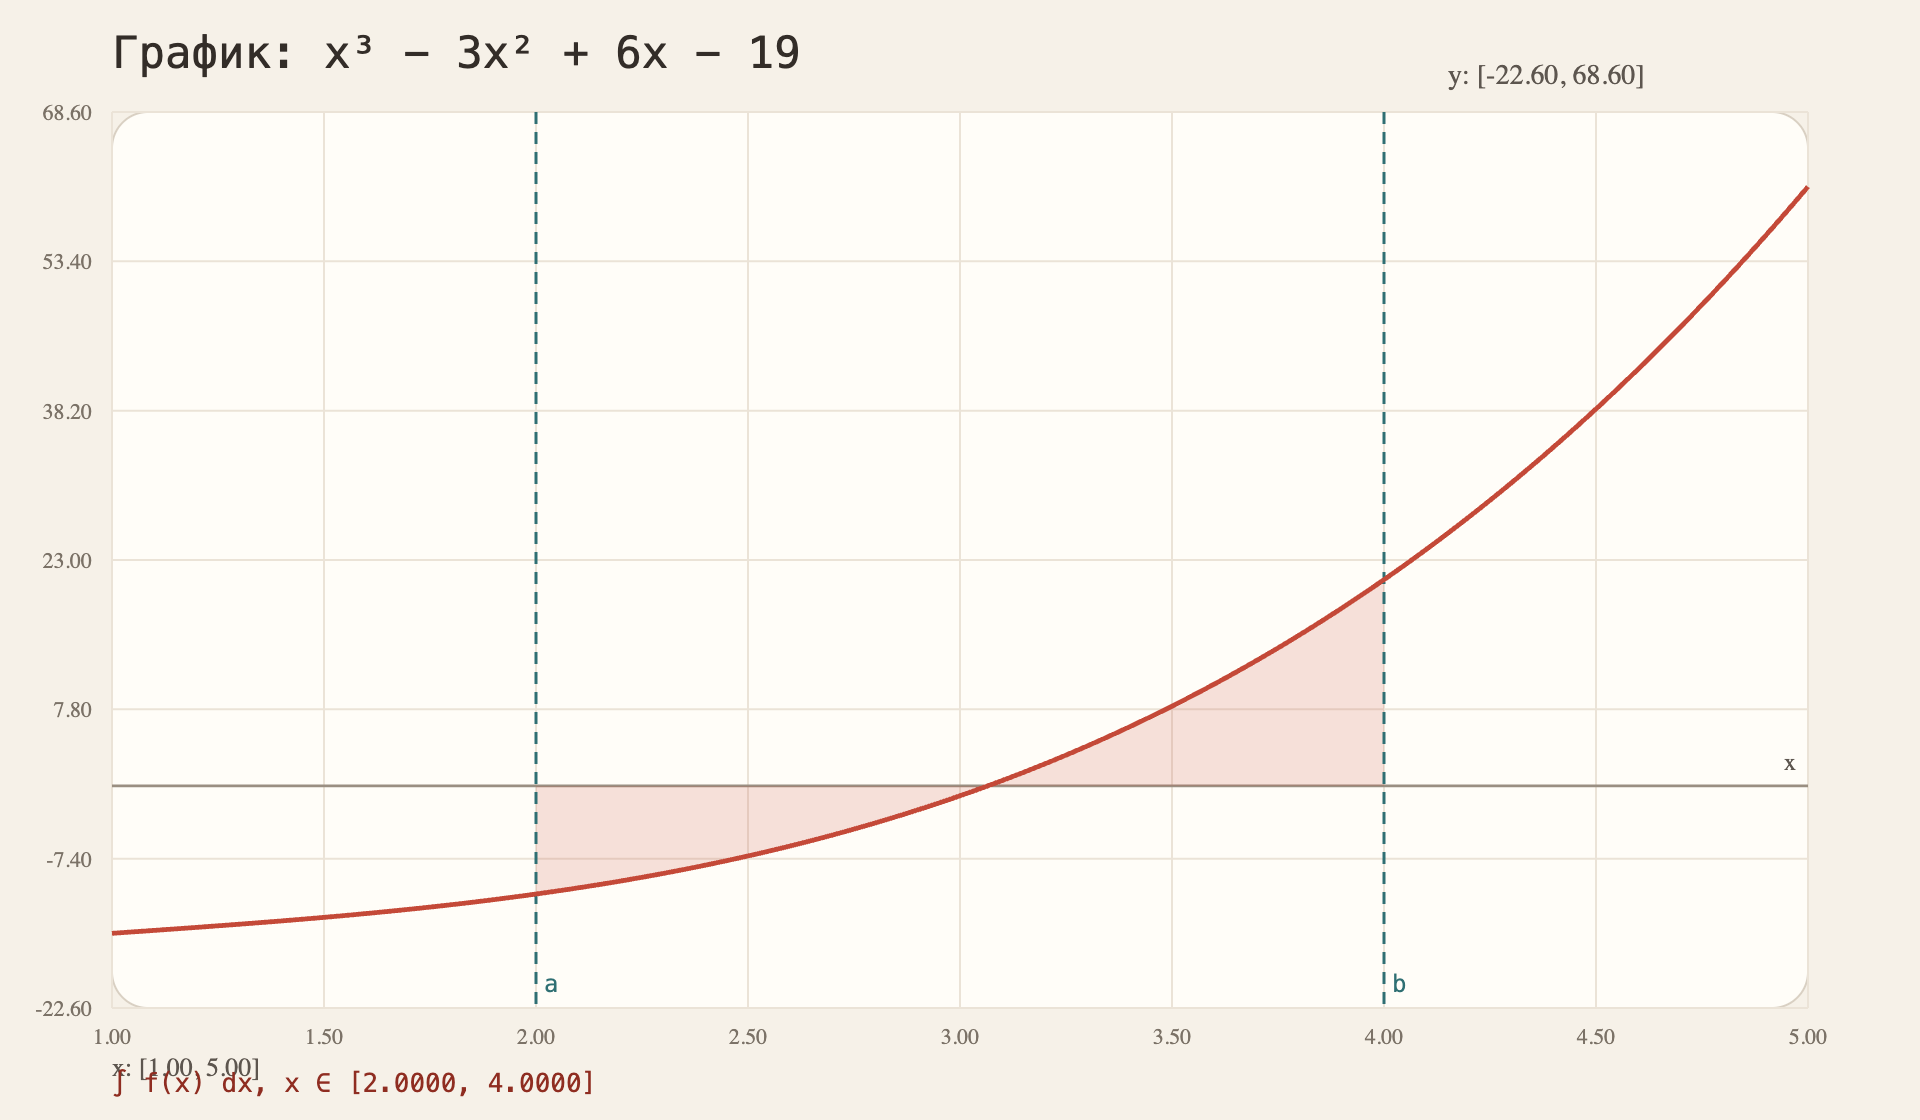
\includegraphics[width=0.96\textwidth]{docs/graph-proper.png}
  \caption{График функции $f(x)=x^{3}-3x^{2}+6x-19$ и площадь интеграла на отрезке $[2;\,4]$}
\end{figure}

На отрезке $[2;\,4]$ функция меняет знак (нуль вблизи $x\approx3.08$), поэтому интеграл
равен разности площадей над и под осью~$Ox$ и принимает небольшое положительное значение.

\subsection{Рабочие формулы методов}

Отрезок $[a,b]$ делится на $n$ равных частей с шагом $h=\dfrac{b-a}{n}$; узлы
$x_i=a+i\,h$, значения $y_i=f(x_i)$, $i=0,1,\dots,n$.

\paragraph{Метод прямоугольников.}
\[
  I_{\text{лев}}=h\sum_{i=0}^{n-1}y_i,\qquad
  I_{\text{прав}}=h\sum_{i=1}^{n}y_i,\qquad
  I_{\text{сред}}=h\sum_{i=1}^{n}f\!\left(x_{i-1/2}\right),\;
  x_{i-1/2}=x_{i-1}+\tfrac{h}{2}.
\]

\paragraph{Метод трапеций.}
\[
  I_{\text{трап}}=h\left(\frac{y_0+y_n}{2}+\sum_{i=1}^{n-1}y_i\right).
\]

\paragraph{Метод Симпсона} (число $n$ чётное):
\[
  I_{\text{Симп}}=\frac{h}{3}\Bigl(y_0+y_n
  +4\,(y_1+y_3+\dots+y_{n-1})
  +2\,(y_2+y_4+\dots+y_{n-2})\Bigr).
\]

\paragraph{Формула Ньютона--Котеса} порядка $n$:
\[
  I=\frac{n\,h}{C_n}\sum_{i=0}^{n}c_n^{\,i}\,f(x_i).
\]
Для $n=6$: $C_6=840$, коэффициенты Котеса $c_6^{\,i}=\{41,\,216,\,27,\,272,\,27,\,216,\,41\}$.

\paragraph{Правило Рунге.}
Оценка погрешности по результатам с шагами $h$ и $h/2$:
\[
  R\approx\frac{\bigl|I_{h/2}-I_{h}\bigr|}{2^{k}-1},
\]
где $k$ — порядок точности метода: $k=1$ для левых и правых прямоугольников, $k=2$ для
средних прямоугольников и трапеций, $k=4$ для метода Симпсона. Число разбиений удваивается,
пока $R>\varepsilon$.

\subsection{Точное значение интеграла}

Первообразная: $F(x)=\dfrac{x^{4}}{4}-x^{3}+3x^{2}-19x$.
\[
  I=F(4)-F(2)=(-28)-(-30)=\boxed{2}.
\]

\subsection{Формула Ньютона--Котеса при $n=6$}

Шаг $h=\dfrac{4-2}{6}=\dfrac{1}{3}$. Значения функции в узлах:

\begin{table}[H]
  \centering
  \caption{Узлы для формулы Ньютона--Котеса ($n=6$)}
  \begin{tabular}{C{1.4cm}C{2.8cm}C{3.2cm}}
    \toprule
    $i$ & $x_i$ & $f(x_i)$ \\
    \midrule
    0 & 2.00000 & $-11.00000$ \\
    1 & 2.33333 & $-8.62963$ \\
    2 & 2.66667 & $-5.37037$ \\
    3 & 3.00000 & $-1.00000$ \\
    4 & 3.33333 & $4.70370$ \\
    5 & 3.66667 & $11.96296$ \\
    6 & 4.00000 & $21.00000$ \\
    \bottomrule
  \end{tabular}
\end{table}

\[
  I_{\text{НК}}=\frac{6\cdot\frac{1}{3}}{840}\sum_{i=0}^{6}c_6^{\,i}f(x_i)
  =\frac{1}{420}\cdot 840 = \boxed{2.00000}.
\]
Для многочлена степени 3 формула Ньютона--Котеса при $n=6$ даёт точное значение.

\subsection{Прямоугольники, трапеции и Симпсон при $n=10$}

Шаг $h=\dfrac{4-2}{10}=0.2$. Значения функции в узлах:

\begin{table}[H]
  \centering
  \caption{Узлы для формул при $n=10$}
  \begin{tabular}{C{1cm}C{1.8cm}C{2.4cm}C{1cm}C{1.8cm}C{2.4cm}}
    \toprule
    $i$ & $x_i$ & $f(x_i)$ & $i$ & $x_i$ & $f(x_i)$ \\
    \midrule
    0 & 2.0 & $-11.000$ & 6 & 3.2 & $2.248$ \\
    1 & 2.2 & $-9.672$ & 7 & 3.4 & $6.024$ \\
    2 & 2.4 & $-8.056$ & 8 & 3.6 & $10.376$ \\
    3 & 2.6 & $-6.104$ & 9 & 3.8 & $15.352$ \\
    4 & 2.8 & $-3.768$ & 10 & 4.0 & $21.000$ \\
    5 & 3.0 & $-1.000$ & & & \\
    \bottomrule
  \end{tabular}
\end{table}

\begin{align*}
  I_{\text{сред}} &= 0.2\sum_{i=1}^{10} f(x_{i-1/2}) = 1.96000, \\
  I_{\text{трап}} &= 0.2\left(\frac{-11+21}{2}+\sum_{i=1}^{9}y_i\right) = 2.08000, \\
  I_{\text{Симп}} &= \frac{0.2}{3}\bigl(y_0+y_{10}+4\textstyle\sum_{\text{нечёт}}y_i+2\sum_{\text{чёт}}y_i\bigr) = 2.00000.
\end{align*}

\subsection{Сравнение результатов и относительная погрешность}

\begin{table}[H]
  \centering
  \caption{Сравнение методов с точным значением $I=2$}
  \begin{tabular}{C{6.8cm}C{3cm}C{3.4cm}}
    \toprule
    \textbf{Метод} & \textbf{Значение} & \textbf{Отн. погрешность} \\
    \midrule
    Точное значение (Ньютон--Лейбниц) & 2.00000 & --- \\
    Ньютон--Котес, $n=6$ & 2.00000 & $0\%$ \\
    Средние прямоугольники, $n=10$ & 1.96000 & $2{,}0000\%$ \\
    Трапеции, $n=10$ & 2.08000 & $4{,}0000\%$ \\
    Симпсон, $n=10$ & 2.00000 & $0\%$ \\
    \bottomrule
  \end{tabular}
\end{table}

% ====================== РАЗДЕЛ 2 ======================
\section{Программная реализация}

Проект написан на JavaScript. Консольная часть запускается через Node.js, для визуализации
дополнительно сделан web-интерфейс в браузере. Вычисление значений функции вынесено в
отдельный класс \texttt{FunctionEvaluator}, каждый метод интегрирования оформлен отдельной
функцией, а число разбиений подбирается автоматически по правилу Рунге (начальное $n=4$).
Пользователь выбирает подынтегральную функцию (пять определённых интегралов и три
несобственных интеграла 2 рода), задаёт пределы $a$, $b$, метод и точность~$\varepsilon$.

\subsection{Листинг программы}

Вычисление значений функции оформлено отдельным классом:

\begin{lstlisting}
export class FunctionEvaluator {
  constructor(definition) { this.definition = definition; }
  evaluate(x) {
    const value = this.definition.f(x);
    if (!Number.isFinite(value)) {
      throw new Error("Function is not defined (infinite discontinuity).");
    }
    return value;
  }
  hasAntiderivative() { return typeof this.definition.F === "function"; }
  exactIntegral(a, b) {
    return this.hasAntiderivative() ? this.definition.F(b) - this.definition.F(a) : null;
  }
}
\end{lstlisting}

Каждый метод интегрирования — отдельная функция:

\begin{lstlisting}
export function leftRectangles(f, a, b, n) {
  const h = (b - a) / n;
  let sum = 0;
  for (let i = 0; i < n; i += 1) sum += f.evaluate(a + i * h);
  return h * sum;
}

export function trapezoidal(f, a, b, n) {
  const h = (b - a) / n;
  let sum = (f.evaluate(a) + f.evaluate(b)) / 2;
  for (let i = 1; i < n; i += 1) sum += f.evaluate(a + i * h);
  return h * sum;
}

export function simpson(f, a, b, n) {
  let segments = n % 2 === 0 ? n : n + 1;
  const h = (b - a) / segments;
  let sum = f.evaluate(a) + f.evaluate(b);
  for (let i = 1; i < segments; i += 1) {
    sum += (i % 2 === 1 ? 4 : 2) * f.evaluate(a + i * h);
  }
  return (h / 3) * sum;
}
\end{lstlisting}

Оценка погрешности и остановка по правилу Рунге (начальное $n=4$):

\begin{lstlisting}
export function integrateWithRunge(methodId, f, a, b, epsilon) {
  const order = meta[methodId].order;        // k: 1, 2 or 4
  const denom = 2 ** order - 1;
  let n = 4;
  let prev = methodFn(f, a, b, n);
  while (true) {
    const nextN = n * 2;
    const curr = methodFn(f, a, b, nextN);
    const runge = Math.abs(curr - prev) / denom;
    if (runge <= epsilon) return { value: curr, n: nextN, runge };
    prev = curr; n = nextN;
  }
}
\end{lstlisting}

\subsection{Результаты выполнения программы}

Автоматический подбор числа разбиений по правилу Рунге для всех методов
(точность $\varepsilon=1\cdot10^{-4}$, начальное $n=4$):

\begin{table}[H]
  \centering
  \caption{Результаты при $\varepsilon=10^{-4}$}
  \begin{tabular}{C{5.4cm}C{2.8cm}C{2.2cm}C{2.8cm}}
    \toprule
    \textbf{Метод} & \textbf{Значение} & \textbf{$n$} & \textbf{Оценка $R$} \\
    \midrule
    Левые прямоугольники & 1.999939 & 524288 & $6{,}1\cdot10^{-5}$ \\
    Правые прямоугольники & 2.000061 & 524288 & $6{,}1\cdot10^{-5}$ \\
    Средние прямоугольники & 1.999939 & 256 & $6{,}1\cdot10^{-5}$ \\
    Метод трапеций & 2.000031 & 512 & $3{,}1\cdot10^{-5}$ \\
    Метод Симпсона & 2.000000 & 8 & $\approx 0$ \\
    \bottomrule
  \end{tabular}
\end{table}

Видно, что метод Симпсона достигает точности уже при $n=8$, средние прямоугольники и
трапеции — при $n=256$ и $n=512$, а левые/правые прямоугольники (первый порядок точности)
требуют $n\approx5\cdot10^{5}$.

\subsection{Несобственные интегралы 2 рода}

Программа определяет сходимость несобственного интеграла 2 рода: усечённый интеграл
$J(\sigma)=\int_{a+\sigma}^{b}f\,dx$ вычисляется численно для убывающих $\sigma$, и если
последовательность $J(\sigma)$ имеет конечный предел, интеграл сходится; иначе выводится
сообщение «Интеграл не существует». Рассмотрены все три случая бесконечного разрыва.

\begin{table}[H]
  \centering
  \caption{Исследование несобственных интегралов 2 рода ($\varepsilon=10^{-3}$)}
  \begin{tabular}{C{3.4cm}C{1.8cm}C{2.6cm}C{2.4cm}C{2.6cm}}
    \toprule
    \textbf{Функция} & \textbf{Отрезок} & \textbf{Особая точка} & \textbf{Сходимость} & \textbf{Значение} \\
    \midrule
    $1/\sqrt{x}$ & $[0;1]$ & $x=a=0$ & сходится & 2.00001 \\
    $1/(1-x)$ & $[0;1]$ & $x=b=1$ & расходится & не существует \\
    $1/\sqrt[3]{(x-2)^2}$ & $[1;3]$ & $x=c=2$ & сходится & 6.00016 \\
    \bottomrule
  \end{tabular}
\end{table}

\subsection{Скриншоты работы программы}

На рисунках ниже показана работа программы: вычисление определённого интеграла варианта 19
и исследование несобственного интеграла 2 рода.

\begin{figure}[H]
  \centering
  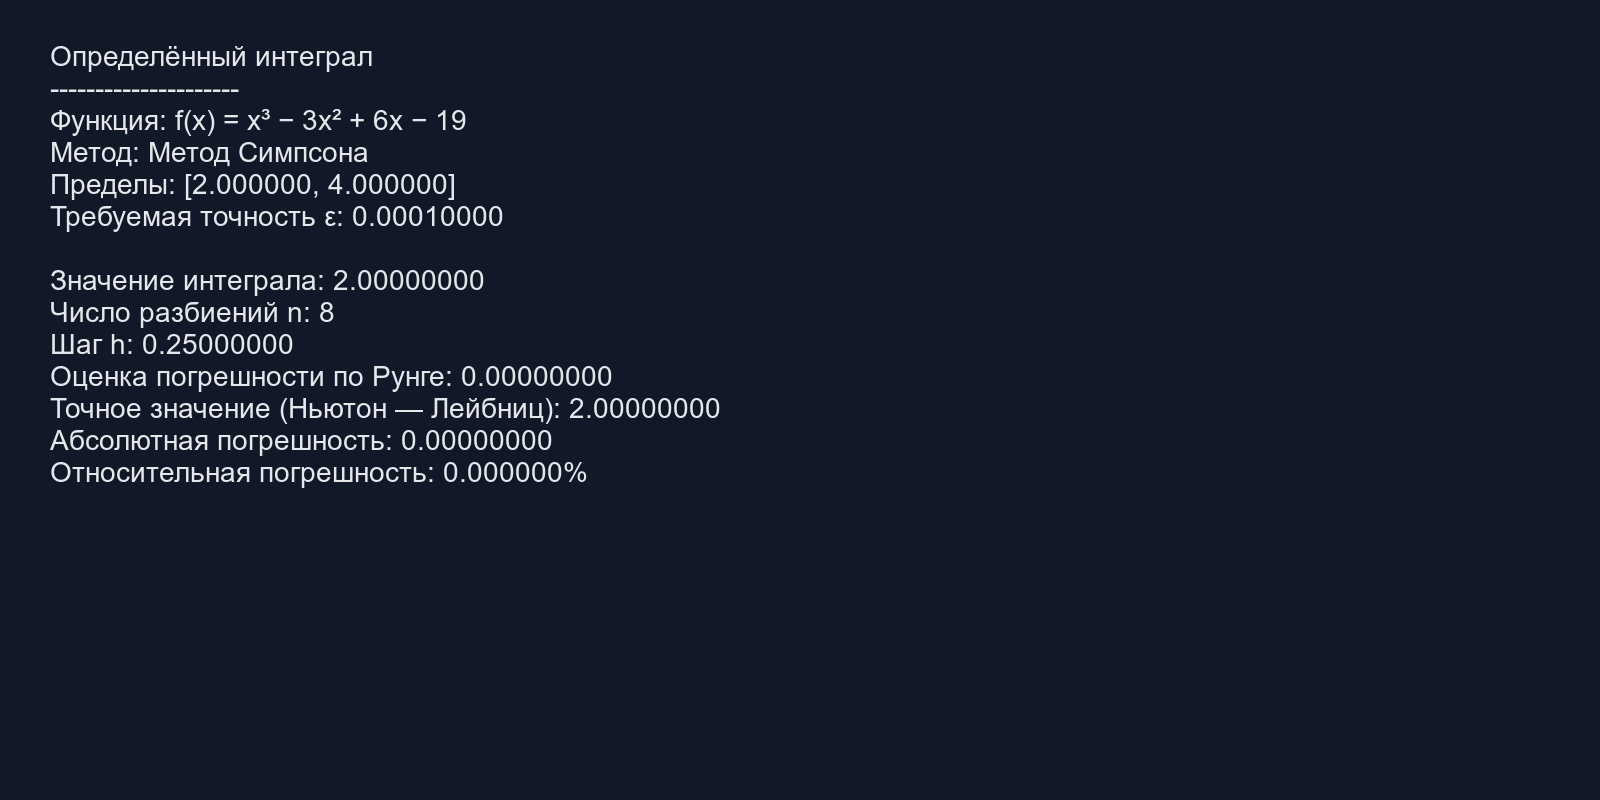
\includegraphics[width=\textwidth,height=0.86\textheight,keepaspectratio]{output/screenshots/console-proper.png}
  \caption{Вычисление определённого интеграла варианта 19 методом Симпсона}
\end{figure}

\begin{figure}[H]
  \centering
  
\includegraphics[width=\textwidth,height=0.86\textheight,keepaspectratio]{output/screenshots/console-improper.png}
  \caption{Исследование несобственного интеграла 2 рода}
\end{figure}

% ====================== РАЗДЕЛ 3 ======================
\section{Вывод}

\begin{itemize}[leftmargin=*]
  \item Формула Симпсона и формула Ньютона--Котеса при $n=6$ для многочлена степени~3 дают
        точное значение интеграла, поскольку точны для многочленов соответствующей степени.
  \item Формулы средних прямоугольников и трапеций имеют второй порядок точности $O(h^2)$;
        при $n=10$ их относительные погрешности составили $2\%$ и $4\%$ соответственно.
        Метод средних прямоугольников вдвое точнее метода трапеций (коэффициенты $\frac{1}{24}$
        против $\frac{1}{12}$ в оценке погрешности).
  \item Левые и правые прямоугольники имеют первый порядок точности и сходятся медленнее
        всего: для $\varepsilon=10^{-4}$ потребовалось $n\approx5\cdot10^{5}$ разбиений.
  \item Правило Рунге позволяет оценивать погрешность и автоматически подбирать число
        разбиений, не вычисляя производных подынтегральной функции.
  \item Для несобственных интегралов 2 рода программа корректно различает сходящиеся и
        расходящиеся интегралы и вычисляет значение сходящихся во всех трёх случаях
        расположения особой точки.
\end{itemize}

\end{document}
